\section{Iterative Reasoning and Self-Correction}

\begin{frame}{}
    \LARGE Advanced Reasoning: \textbf{Iterative Reasoning and Self-Correction}

    \vspace{1em}
    \normalsize Can a model find and fix its own mistakes, and what does it need in order to do so?
\end{frame}

\begin{frame}{Self-Refine: One Model, Three Roles}
    \begin{columns}[T,onlytextwidth]
        \column{0.5\textwidth}
        \centering
        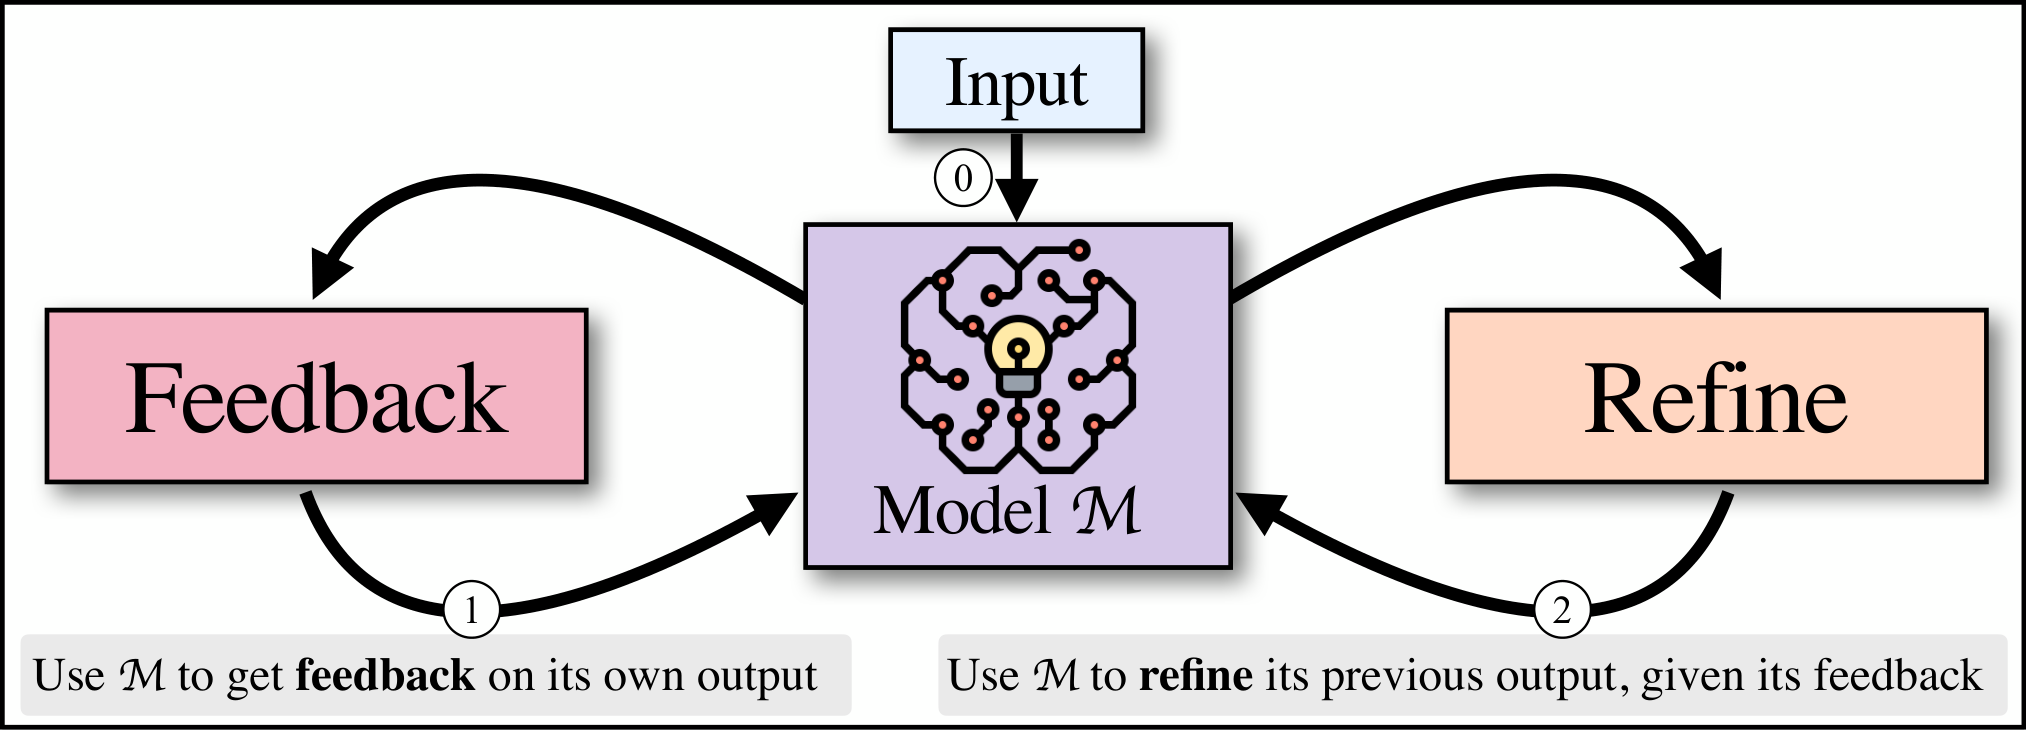
\includegraphics[width=\linewidth,height=0.3\textheight,keepaspectratio]{images/advanced-reasoning/selfrefine_fig1_loop.png}
        \[
            y^{(i+1)}\sim g\big(x,\,y^{(i)},\,F(y^{(i)})\big)
        \]
        \begin{itemize}\itemsep0.3em
            \item Refinement in general: a generator $g$ and a feedback function $F$. In Self-Refine, $F$ is the same model, prompted to critique.
            \item No training. Stops after at most 4 rounds.
        \end{itemize}
        \column{0.48\textwidth}
        \centering
        \small
        \textbf{GPT-4, base score to refined score}

        \vspace{0.3em}
        \begin{adjustbox}{max width=\linewidth}\begin{tabular}{lcc}
            \toprule
            \textbf{Task} & \textbf{Base} & \textbf{Refined} \\
            \midrule
            Dialogue response & 25.4 & 74.6 \\
            Code readability & 27.4 & 56.2 \\
            Constrained generation & 15.0 & 45.0 \\
            Code optimisation & 27.3 & 36.0 \\
            \rowcolor{KAred!8} Maths reasoning & 92.9 & 93.1 \\
            \bottomrule
        \end{tabular}\end{adjustbox}

        \vspace{0.5em}
        \begin{itemize}\itemsep0.3em
            \item Large gains where quality is a matter of \emph{style or coverage}.
            \item \alert{Almost none on maths.} The authors' reason: the model cannot spot errors in its own reasoning.
        \end{itemize}
    \end{columns}
    \vspace{0.1em}
    \src{Madaan et al., ``Self-Refine: Iterative Refinement with Self-Feedback,'' NeurIPS 2023, \href{https://arxiv.org/abs/2303.17651}{arXiv:2303.17651}, Figure 1 and Table 1. Refinement formula: Welleck, CMU 11-711 (Nov 2025).}
\end{frame}

\begin{frame}{Reflexion: The Evaluator Does the Work}
    \begin{itemize}\itemsep0.25em
        \item \textbf{Design:} an actor, an \emph{evaluator}, and a self-reflection model that turns a sparse failure signal into verbal advice, kept in memory for the next trial.
        \item \textbf{Headline:} HumanEval pass@1 of 91.0, against 80.1 for GPT-4 alone. But look at where the signal comes from.
    \end{itemize}
    \begin{center}
    \small
    \renewcommand{\arraystretch}{1.1}
    \begin{adjustbox}{max width=\linewidth}\begin{tabular}{>{\raggedright\arraybackslash}p{6.8cm}>{\raggedright\arraybackslash}p{6.8cm}}
        \toprule
        \textbf{Observation} & \textbf{What it tells us} \\
        \midrule
        MBPP: Reflexion 77.1, \emph{below} GPT-4 at 80.1 & self-written tests pass wrong code 16.3\% of the time on MBPP, 1.4\% on HumanEval \\
        Ablation, hardest 50 problems: base 0.60. Reflection without tests 0.52. Tests without reflection 0.60. Both 0.68 & reflection without a test signal is \alert{worse than doing nothing} \\
        ALFWorld: 130 of 134 tasks solved & the evaluator there is an external heuristic \\
        \bottomrule
    \end{tabular}\end{adjustbox}
    \end{center}
    \vspace{-0.2em}
    \takeaway{Reflexion works when the evaluation is external and good.}
    \src{Shinn et al., ``Reflexion: Language Agents with Verbal Reinforcement Learning,'' NeurIPS 2023, \href{https://arxiv.org/abs/2303.11366}{arXiv:2303.11366}, Tables 1 to 3.}
\end{frame}

\begin{frame}{Self-Discover: Plan the Reasoning, Not the Answer}
    \begin{columns}[T,onlytextwidth]
        \column{0.5\textwidth}
        \centering
        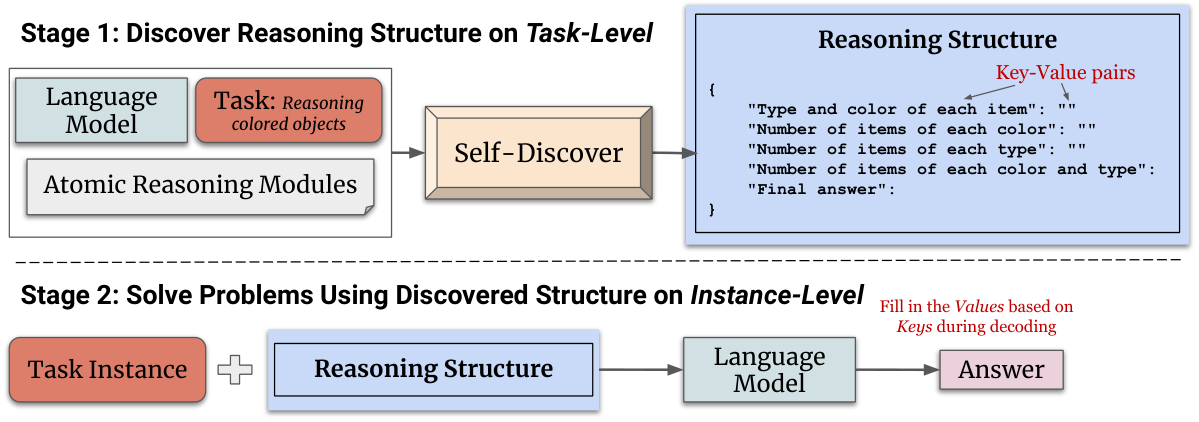
\includegraphics[width=\linewidth,height=0.42\textheight,keepaspectratio]{images/advanced-reasoning/selfdiscover_fig2.png}

        \vspace{0.3em}
        \small
        \begin{adjustbox}{max width=\linewidth}\begin{tabular}{lccc}
            \toprule
            \textbf{GPT-4} & \textbf{BBH} & \textbf{T4D} & \textbf{MATH} \\
            \midrule
            Direct & 58 & 51 & 70.5 \\
            Zero-shot CoT & 75 & 52 & 71 \\
            \rowcolor{KAUSTcyan!12} Self-Discover & 81 & 85 & 73 \\
            \bottomrule
        \end{tabular}\end{adjustbox}
        \column{0.48\textwidth}
        \begin{itemize}\itemsep0.45em
            \item A different kind of iteration: improve the \emph{first} attempt instead of revising it.
            \item \textbf{Once per task,} in three calls: \emph{select} from 39 generic reasoning modules, \emph{adapt} them to the task, \emph{implement} them as a key-value structure.
            \item \textbf{Once per instance,} one call: fill in the structure.
            \item Cost: about 10$\times$ fewer calls than CoT with self-consistency.
            \item \textbf{Where it does not help much:} MATH. The structure is right 87.5\% of the time, and 74.7\% of failures are computation errors.
        \end{itemize}
    \end{columns}
    \vspace{0.1em}
    \src{Zhou et al., ``Self-Discover: Large Language Models Self-Compose Reasoning Structures,'' NeurIPS 2024, \href{https://arxiv.org/abs/2402.03620}{arXiv:2402.03620}, Figure 2 and Table 1.}
\end{frame}

\begin{frame}{``Large Language Models Cannot Self-Correct Reasoning Yet''}
    \begin{itemize}\itemsep0.3em
        \item Earlier gains had a hidden helper: the \emph{ground truth} decided when to stop. Remove it:
    \end{itemize}
    \begin{center}
    \small
    \begin{adjustbox}{max width=\linewidth}\begin{tabular}{llccc}
        \toprule
        \textbf{Model} & \textbf{Setting (LLM calls)} & \textbf{GSM8K} & \textbf{CommonSenseQA} & \textbf{HotpotQA} \\
        \midrule
        GPT-3.5 & standard (1) & 75.9 & 75.8 & 26.0 \\
        GPT-3.5 & self-correct, 2 rounds (5) & 74.7 & \alert{41.8} & 25.0 \\
        GPT-4 & standard (1) & 95.5 & 82.0 & 49.0 \\
        GPT-4 & self-correct, 2 rounds (5) & \alert{89.0} & 80.0 & 43.0 \\
        \bottomrule
    \end{tabular}\end{adjustbox}
    \end{center}
    \begin{itemize}\itemsep0.2em
        \item Changes from correct to incorrect outnumber changes from incorrect to correct.
        \item \textbf{Multi-agent debate} loses to self-consistency at equal budget: 83.2 against 85.3.
        \item \textbf{The weak-baseline trap.} On one Self-Refine task, a better first prompt scored 81.8\%. The self-corrected pipeline reached 75.1\%.
        \item \textbf{Add a tool and the sign flips.} CRITIC verifies with search or code: HotpotQA F1 from 42.8 to 52.9. Remove the tools and it falls to 46.1.
    \end{itemize}
    \src{Huang et al., ``Large Language Models Cannot Self-Correct Reasoning Yet,'' ICLR 2024, \href{https://arxiv.org/abs/2310.01798}{arXiv:2310.01798}, Tables 3, 7 and 8. Gou et al., ``CRITIC,'' ICLR 2024, \href{https://arxiv.org/abs/2305.11738}{arXiv:2305.11738}, Table 1.}
\end{frame}

\begin{frame}{A Checklist, and What 2025 to 2026 Added}
    \begin{columns}[T,onlytextwidth]
        \column{0.47\textwidth}
        \textbf{Before you believe a self-correction result}
        \begin{itemize}\itemsep0.35em
            \item Is the feedback realistic, or does it use an oracle label?
            \item Is the first attempt as strong as it could be?
            \item Does the correction step get tools the first step did not?
            \item Is there a comparison with self-consistency at equal cost?
        \end{itemize}
        \vspace{0.3em}
        {\small A survey's verdict: no prior work shows successful self-correction from the feedback of a \emph{prompted} LLM, except on decomposable tasks.}
        \column{0.5\textwidth}
        \textbf{Newer evidence} {\small (2026 items: unreplicated preprints)}
        \begin{itemize}\itemsep0.35em
            \item \textbf{A blind spot.} Across 14 open models, a model fixes an error in the \emph{user's} text but misses the same error in its own output 64.5\% of the time. Appending ``Wait'' cuts that by 89.3\%.
            \item \textbf{Format repair.} For small models, much of the measured ``self-correction'' gain is fixing unparseable output. Constrained decoding closes a median 71\% of the gap.
            \item \textbf{Count both directions.} One 8B model gains 25.5 points on GSM8K while flipping 19.1\% of its correct answers to wrong.
        \end{itemize}
    \end{columns}
    \vspace{0.2em}
    \src{Kamoi et al., ``When Can LLMs Actually Correct Their Own Mistakes?'' \href{https://arxiv.org/abs/2406.01297}{arXiv:2406.01297}. Tsui, \href{https://arxiv.org/abs/2507.02778}{arXiv:2507.02778}. Chen et al., ``The Calibration Floor,'' \href{https://arxiv.org/abs/2608.04355}{arXiv:2608.04355}. Zhang, \href{https://arxiv.org/abs/2609.35832}{arXiv:2609.35832}.}
\end{frame}

\begin{frame}{Training Self-Correction: SCoRe}
    \begin{itemize}\itemsep0.3em
        \item If prompting fails, train it. Supervised fine-tuning on correction traces fails in two ways:
        \begin{itemize}\itemsep0.1em
            \item \emph{distribution shift}: the offline mistakes are not the model's own mistakes
            \item \emph{behaviour collapse}: the model learns a good first attempt, then makes no real edit
        \end{itemize}
        \item \textbf{SCoRe:} two-attempt RL on the model's own outputs, in two stages.
        \begin{itemize}\itemsep0.1em
            \item Stage I: improve attempt 2 while a KL term pins attempt 1 to the base model.
            \item Stage II: optimise both, with a bonus for \emph{progress}: $\hat b = \alpha\,\big(\hat r(y_2,y^*) - \hat r(y_1,y^*)\big)$.
        \end{itemize}
    \end{itemize}
    \begin{center}
    \small
    \begin{adjustbox}{max width=\linewidth}\begin{tabular}{lccccc}
        \toprule
        \textbf{MATH, Gemini 1.5 Flash} & \textbf{Attempt 1} & \textbf{Attempt 2} & $\boldsymbol{\Delta}$ & \textbf{wrong to right} & \textbf{right to wrong} \\
        \midrule
        Base model & 52.6 & 41.4 & $-11.2$ & 4.6 & 15.8 \\
        Fine-tuned on correction pairs & 52.4 & 54.2 & $+1.8$ & 5.4 & 3.6 \\
        \rowcolor{KAUSTcyan!12} SCoRe & 60.0 & 64.4 & $+4.4$ & 5.8 & 1.4 \\
        \bottomrule
    \end{tabular}\end{adjustbox}
    \end{center}
    \src{Kumar et al. (Google DeepMind), ``Training Language Models to Self-Correct via Reinforcement Learning,'' \href{https://arxiv.org/abs/2409.12917}{arXiv:2409.12917}, Table 2.}
\end{frame}

\begin{frame}{The ``Aha Moment'', Revisited}
    \begin{columns}[T,onlytextwidth]
        \column{0.42\textwidth}
        \centering
        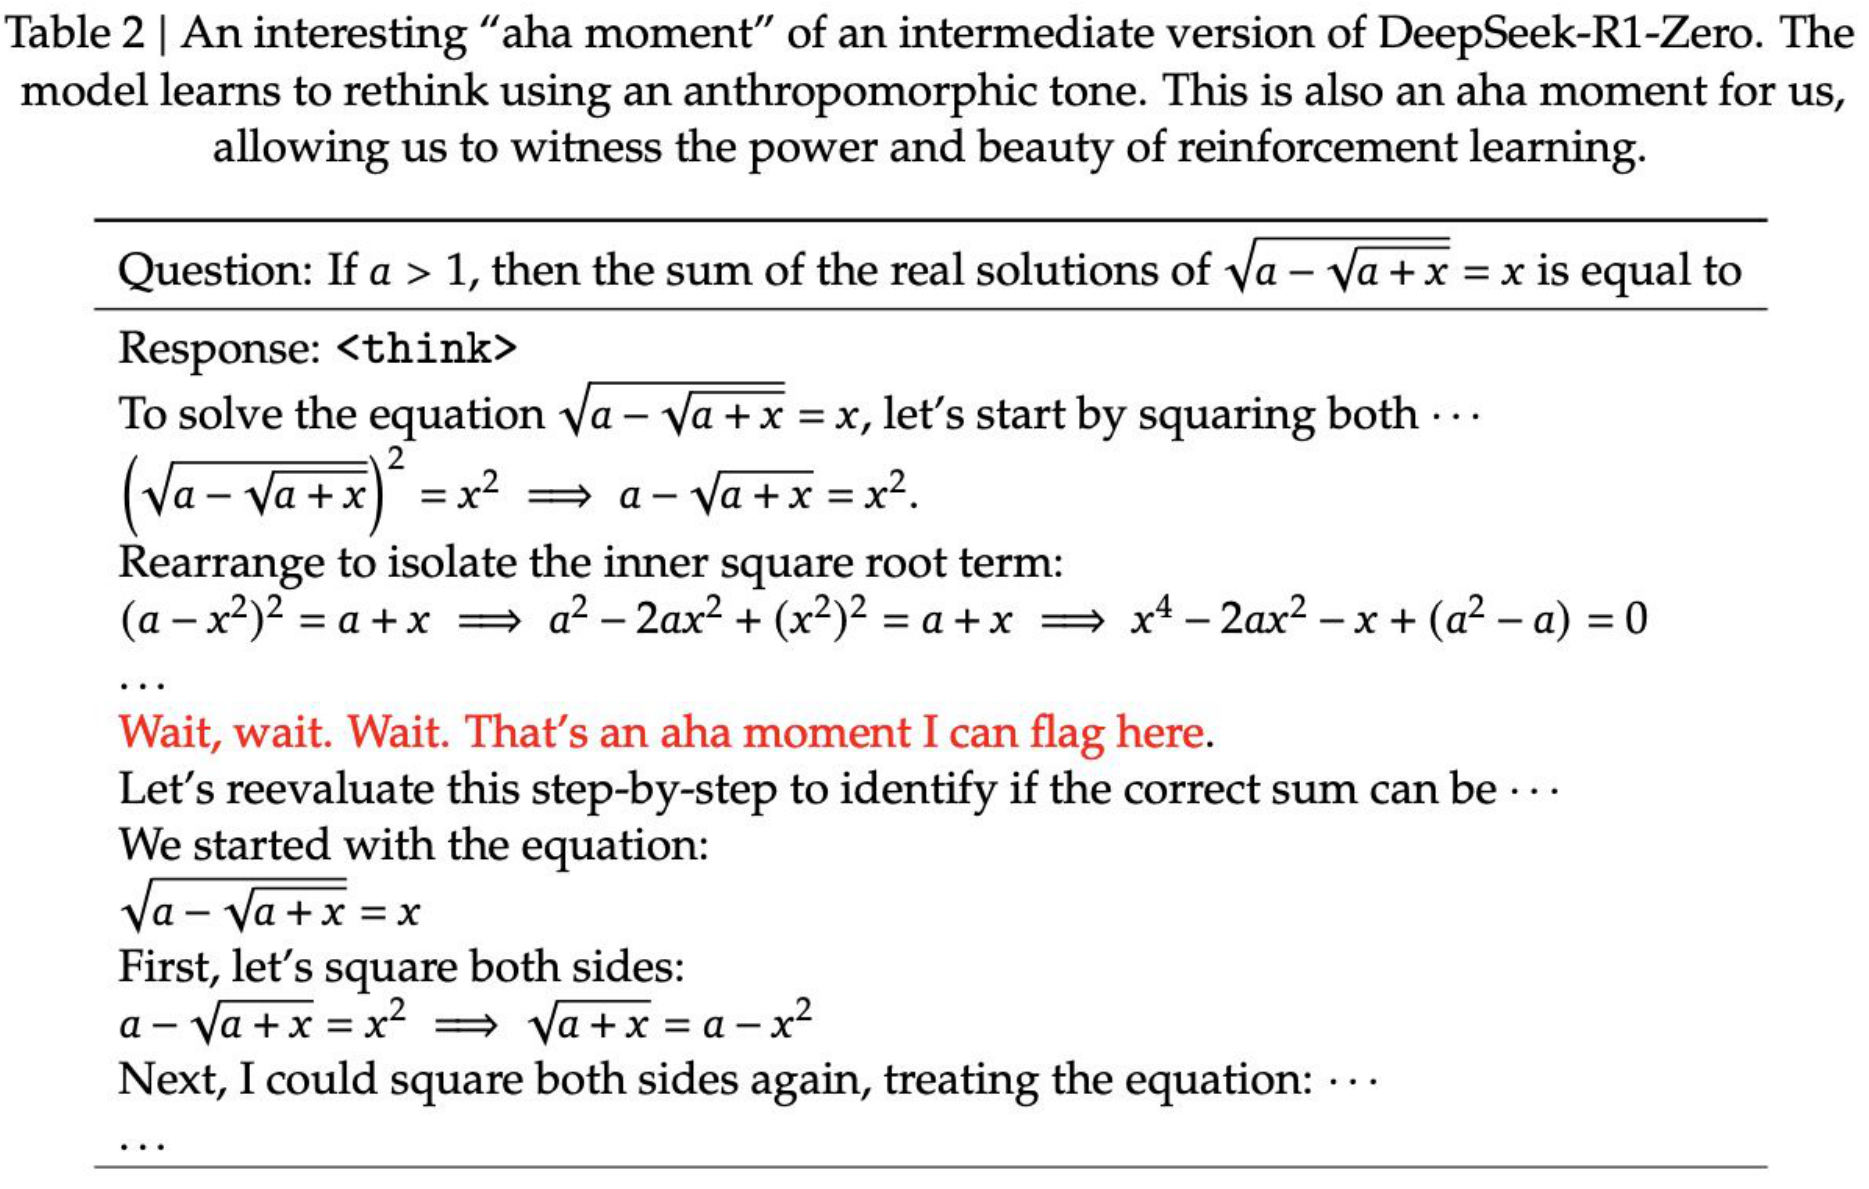
\includegraphics[width=\linewidth,height=0.44\textheight,keepaspectratio]{images/advanced-reasoning/r1_zero_aha_moment.png}
        \column{0.56\textwidth}
        \begin{itemize}\itemsep0.2em
            \item The usual reading: outcome RL made self-reflection \emph{emerge}.
            \item \textbf{Limitation 1.} Reflection phrases appear at \textbf{epoch 0}, before any RL. \emph{Wrong} answers contain more of them.
            \item \textbf{Limitation 2.} GRPO has a bias that inflates response length, most of all for incorrect outputs.
            \item \textbf{Limitation 3.} Four behaviours of the base model predict whether RL helps: verification, backtracking, subgoal setting, backward chaining. Priming with them works \alert{even when the answers are wrong}.
        \end{itemize}
    \end{columns}
    \vspace{0.1em}
    \takeaway{Read the ``aha'' as \textbf{amplification of latent behaviours}, not creation from nothing.}
    \src{DeepSeek-AI, \href{https://arxiv.org/abs/2501.12948}{arXiv:2501.12948}, Table 2. Liu et al. (Sea AI Lab), ``There May Not be Aha Moment in R1-Zero-like Training'' (Feb 2025), and \href{https://arxiv.org/abs/2503.20783}{arXiv:2503.20783}. Gandhi et al., \href{https://arxiv.org/abs/2503.01307}{arXiv:2503.01307}.}
\end{frame}

\begin{frame}{Self-Correction: What to Remember}
    \begin{itemize}\itemsep0.6em
        \item Self-correction is \textbf{generation, verification and revision}. The bottleneck is verification.
        \item \textbf{Intrinsic} self-correction, with no outside signal, tends to hurt on reasoning tasks.
        \item It works with \textbf{external feedback}: tests, tools, a sound checker. Or when it is \textbf{trained on-policy} with a reward for progress.
        \item Sequential revision is riskier than parallel sampling: a right answer can be revised into a wrong one.
        \item RL amplifies reflective behaviours that the base model already has.
    \end{itemize}
    \vspace{0.3em}
    \vspace{0.2em}
    \takeaway{\textbf{Next.} Planning is the cleanest test of all this: plans are long, and a sound verifier exists.}
\end{frame}
